\section{Einleitung}
\subsection{Motivation}
\begin{frame}
\frametitle{Motivation}
\begin{itemize}
\item Große Anwendungsbreite von organischen Halbleitern
\item Polyacetylen als einfaches Testsystem
\item 1950-er \textsc{Longuet-Higgins}: Alternierende Bindungslängen
\item 1980-er \textsc{Su, Schrieffer, Heeger}: Anregungen (Soliton)
\item Gute Bandstruktur mit Tight-Binding
\end{itemize}

\centering
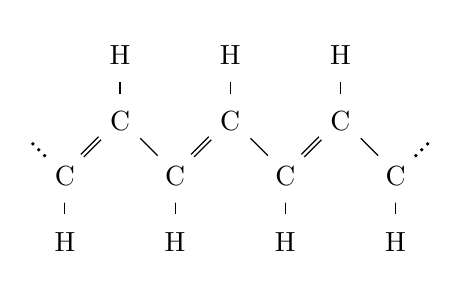
\begin{tikzpicture}[scale = .7]
		\foreach \i in {0,2,4}{
			\draw (\i, 0) -- +(1,1);
			\draw (\i, 0.1) -- +(1,1);
			\draw (\i + 1, 1.05) -- +(1, -1);
			\draw (\i, 0) -- +(0,-.7) node[circle, fill = white, below] {H};
			\draw (\i + 1, 1) -- +(0,.7) node[circle, fill = white, above] {H};
			\node[circle, fill = white] (d\i) at (\i, 0) {C};
			\node[circle, fill = white] (u\i) at (\i + 1, 1) {C};
			}
		\draw (6, 0) -- +(0,-.7) node[circle, fill = white, below] {H};
		\node[circle, fill = white] (end) at (6,0) {C};
		\draw [dotted, line width = 1] (end) -- +(.65,.65);
		\draw [dotted, line width = 1] (d0) -- +(-.65,.65);
\end{tikzpicture}
\end{frame}

\subsection{Dichtefunktionaltheorie}
\begin{frame}
\frametitle{Dichtefunktionaltheorie}
\begin{itemize}
\item Numerische, ab initio, Selbstkonsistenz-Methode zur Berechnung von quantenmechanischen Grundzuständen
\item \textsc{Born-Oppenheimer}-Näherung
\item \textsc{Hohenberg-Kohn} Theoreme:\\
Elektronendichte des Grundzustands bestimmt externes Potential eindeutig und damit Grundzustands-Wellenfunktion:
\begin{align*}
\Psi_0 &= \Psi\left[n_0\right]
\end{align*}
Die Grundzustandsdichte minimiert das Energie-Funktional:
\begin{align*}
E[n_0] &\le E[n]
\end{align*}
\end{itemize}
\end{frame}

\begin{frame}
\begin{itemize}
\item Nicht wechselwirkende Elektron-Wellenfunktionen $\varphi_i$  (\textsc{Kohn-Sham}-Orbitale) mit selber Elektronendichte
\begin{align*}
n(\vec{r}) &= \sum_i \left|\varphi_i\right|^2
\end{align*}
und Einteilchen-Hamiltonian:
\begin{align*}
\mathcal{H} &= \frac{\vec{p}^2}{2m} + V_\text{eff}(\vec{r}, n(\vec{r}))
\end{align*}
\item Unbekannte Terme in $V_\text{eff}(\vec{r}, n(\vec{r}))$: exchange-correlation-Term\\
Verwendete Approximation: PBE (GGA)
\item Lösen mit Iteration und Test auf Selbstkonsistenz
\end{itemize}
\end{frame}


\subsection{Dichtefunktionaltheorie mit Zwangsbedingungen}
\begin{frame}{Dichtefunktionaltheorie mit Zwangsbedingungen (cDFT)}
\hspace*{-1cm}
\begin{minipage}{0.8\textwidth}
	\vspace*{-1.5cm}
	\begin{itemize}
		\item Manuelles Verschieben von Ladung mittels externen Potentialen
		\item Definiere $i$ Regionen und Ladungen $N_i$
		\item Überlagerte Gauß-Kurven $w(\vec{r})$ zentriert an Kernpositionen $\vec{R}_j$
	\end{itemize}
\end{minipage}
\begin{minipage}{0.25\textwidth}
	\vspace*{-.8cm}
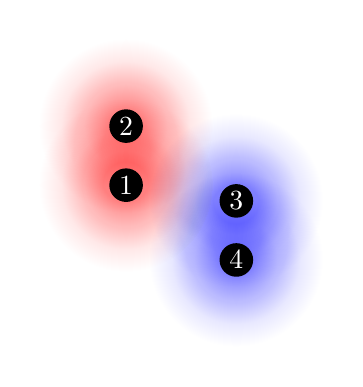
\begin{tikzpicture}[scale = 0.5]
	\foreach \i/\j/\color in {0/0.2/red, 0/1.7/red, 2.8/-0.2/blue, 2.8/-1.7/blue}{
		\foreach \r in {0, 0.01, ..., 1}{
			\fill[opacity = \r * 0.017, fill = \color] (\i, \j) circle ({2.5 * (1 - \r)});}}
	\foreach \i/\j/\num in {0/0.2/1, 0/1.7/2, 2.8/-0.2/3, 2.8/-1.7/4}{
		\node[fill = black, shape = circle, text = white, inner sep = 0.05cm] at (\i, \j)	 {\num};}
\end{tikzpicture}
\end{minipage}
\hspace*{-1cm}
\begin{minipage}{\textwidth}
\vspace*{-1cm}
\begin{itemize}
	\item Test
	\begin{align*}
	F\left[n\left(\vec{r}\right), U_i\right] &= E_0\left[n\left(\vec{r}\right)\right] + 
	\sum_i U_i\left(\int\dd\vec{r}\ w_i\left(\vec{r}\right)\ n\left(\vec{r}\right) - N_i\right)
	\end{align*}
	\item Test
	\begin{align*}
	0 &= \int\dd\vec{r}\ w_i\left(\vec{r}\right)\ n\left(\vec{r}\right) - N_i
	\end{align*}
\end{itemize}
\end{minipage}
\end{frame}